\documentclass{standalone}
\usepackage{tikz}
\usepackage{ctex,siunitx}
\setCJKmainfont{Noto Serif CJK SC}
\usepackage{tkz-euclide}
\usepackage{amsmath,mhchem}
\usetikzlibrary{patterns, calc}
\usetikzlibrary {decorations.pathmorphing, decorations.pathreplacing, decorations.shapes}
\newcommand{\bulb}[1][]{
  \begin{scope}[#1]
    \draw[left color=brown,right color=brown,middle color=white](-0.3,0)rectangle(0.3,-0.1);
    \draw[left color=darkgray,right color=darkgray,middle color=white](-0.1,0.15)rectangle(0.1,0);
    \draw[very thin](-0.05,0.15)--(-0.05,0.3)--(-0.08,0.4)(0.05,0.15)--(0.05,0.3)--(0.08,0.4);
    \draw[very thin,decorate,decoration={zigzag,segment length=1pt,amplitude=0.5pt}](-0.08,0.4)--(0.08,0.4);
    \draw[fill=cyan!20!white,fill opacity=0.3](-0.1,0.15)--(-0.1,0.25)arc(240:-60:0.2)--(0.1,0.15);
    \draw[semithick](-0.2,0)--(-0.2,0.05)(0.2,0)--(0.2,0.05);
    \draw[line cap=round,very thick](-0.2,0.1)--(-0.2,0.05)(0.2,0.1)--(0.2,0.05);
  \end{scope}
}
\newcommand{\retortstand}[4][]{
  \begin{scope}[#1]
    \draw[fill=darkgray](0,0)--++(#3,0)--++(0.05,-0.05)--++(0,-0.15)--++(-0.4,0)--++(0,0.05)--++(-#2-#3+0.7,0)--++(0,-0.05)--++(-0.4,0)--++(0,0.15)--++(0.05,0.05)--cycle;
    \draw(-#2-0.05,-0.05)--(#3+0.05,-0.05);
    \fill[left color=lightgray,right color=lightgray,middle color=white](-0.05,0)rectangle(0.05,#4);
    \fill[left color=gray,right color=gray,middle color=white](-0.07,0)rectangle(0.07,0.07);
  \end{scope}
}
\newcommand{\beaker}[5][]{
  \begin{scope}[#1]
    \fill[#5,rounded corners=1mm](-#2/2,#4)--(-#2/2,0)--(#2/2,0)--(#2/2,#4);
    \draw[fill=cyan!10!white,fill opacity=0.3](#2/2+0.07,#3)arc(90:180:0.07)[rounded corners=1mm]--(#2/2,0)--(-#2/2,0)[rounded corners=0.5mm]--(-#2/2,#3-0.15)[sharp corners]--++(-0.1,0.1)--(-#2/2,#3)--cycle;
  \end{scope}
}
\newcommand{\JointClipC}[3][]{
  \begin{scope}[#1]
    \fill[top color=gray,bottom color=gray,middle color=white](-0.2,-0.03)rectangle(#2,0.03);
    \fill[lightgray](#2,-0.07)rectangle++(#3,0.14);
    \fill[left color=darkgray,right color=darkgray,middle color=white](-0.1,-0.1)rectangle(0.1,0.1);
    \draw[line cap=round,very thick](-135:0.07)--(45:0.07);
    \fill[ball color=black](0,0)circle(1.4pt);
  \end{scope}
}
\begin{document}
\small
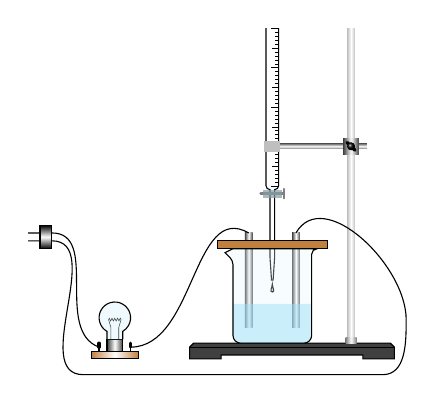
\begin{tikzpicture}[scale=1.0]
  \bulb[xshift=-3cm,yshift=-1mm]
  \retortstand{2}{0.5}{4}
  \draw(-1.08,4)--(-1.08,2.0)arc(180:270:0.05)--(-1.03,1.1)--(-1.01,0.8)--(-0.99,0.8)--(-0.97,1.1)--(-0.97,1.95)arc(-90:0:0.05)--(-0.92,4);
  \foreach \x in {2,2.5,3,3.5}
  {
    \foreach \y in {1,2,3,4,6,7,8,9}
    {\draw[ultra thin](-0.92,\x+0.05*\y)--++(-0.05,0);}
    \draw[ultra thin](-0.92,\x+0.25)--++(-0.08,0);
    \draw[ultra thin](-0.92,\x)--++(-0.1,0);
    \draw[ultra thin](-0.92,\x+0.5)--++(-0.1,0);
  }
  \draw[thick,gray,line cap=round](-1.15,1.9)--(-0.85,1.9)(-0.85,1.84)--(-0.85,1.96);
  \fill[cyan!20!gray,fill opacity=0.7](-1.12,1.95)rectangle(-0.88,1.85);
  \draw[fill=cyan!30!white](-1,0.75)to[out=-90,in=180](-1,0.65)to[out=0,in=-90]cycle;
  \foreach \x in {-1.3,-0.7}
  {
    \fill[left color=darkgray,right color=darkgray,middle color=white](\x-0.05,1.4)rectangle++(0.1,-1.2);
  }
  \draw[fill=brown](-1.7,1.2)rectangle(-0.3,1.3);
  \draw(-0.7,1.4)to[out=60,in=90](0.7,0.3)to[in=0,out=-90](0.4,-0.4)--(-3.4,-0.4)to[out=180,in=0](-3.8,1.3)--++(-0.3,0);
  \draw(-1.3,1.4)to[out=150,in=0](-2.8,-0.05);
  \draw(-3.2,-0.05)to[out=160,in=0](-3.8,1.4)--++(-0.3,0);
  \draw[top color=black,bottom color=black,middle color=white](-3.8,1.2)rectangle(-3.95,1.5);
  \beaker[xshift=-1.0cm]{1.0}{1.2}{0.5}{cyan!50!white,fill opacity=0.5}
  \JointClipC[yshift=2.5cm,xscale=-1]{0.9}{0.2}
\end{tikzpicture}
\end{document}